\newpage
\section{Experiment 6 and 7 - Multiobjective EA}
\label{sec:exp7and7}
To counteract on the diversity problem and the strong bias of the complexity measure (role count, assignments counts), the Evo-RoleMiner$M$ is tested. For the objectives "Minimizing Confidentiality Violations" and "Minimizing Availability Violations" are chosen. The setup can be seen in Table \ref{tab:setup4}.

\begin{table}[H]
	\centering
	\begin{tabular}{|l|l|}
		\hline
		\rowcolor{myGray} 
		\textbf{Parameter}              & \textbf{Value}    \\ \hline
		Generations                     & 100 / 1000       	\\ \hline
		Population                      & 100 / 1000        \\ \hline
		CXPB                            & 0.25              \\ \hline
		MUTPB-Type1: Add role           & 0.25              \\ \hline
		MUTPB-Type2: Add User           & 0.25              \\ \hline
		MUTPB-Type3: Add Permission     & 0.25              \\ \hline
		MUTPB-Type4: Remove Role        & 0.25              \\ \hline
		MUTPB-Type5: Remove User        & 0.25              \\ \hline
		MUTPB-Type6: Remove Permission  & 0.25              \\ \hline
		Local optimization              & True        		\\ \hline
		Objective 1					    & Confidentiality   \\ \hline
		Objective 2					    & Availability     	\\ \hline
	\end{tabular}
	\caption{EXPERIMENT 6 and 7 setup}
	\label{tab:setup4}
\end{table}

The results for the synthetic dataset 1 are illustrated in Figure \ref{fig:exp6_fitness} and \ref{fig:exp6_measures}. For the healthcare dataset the results can be seen in Figure \ref{fig:exp7_fitness} and \ref{fig:exp7_measures}.

\begin{figure}[H]
	\centering
	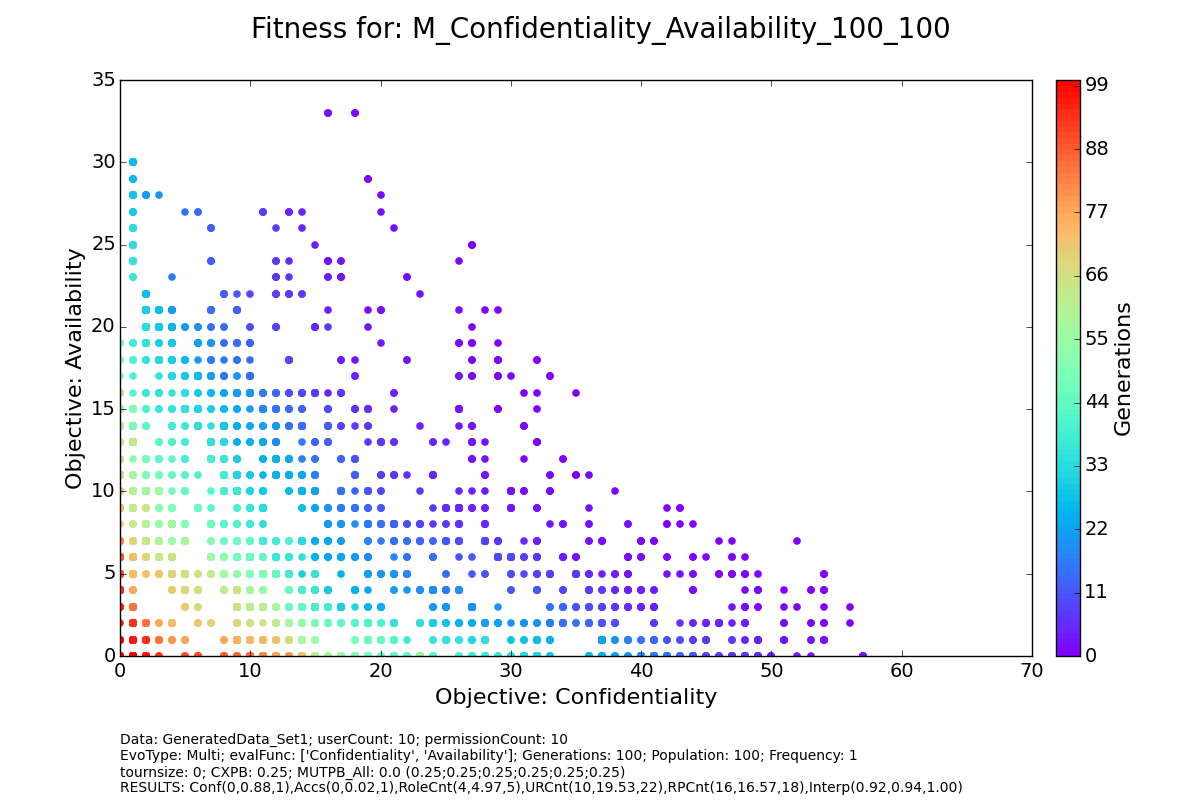
\includegraphics[scale=0.35, trim=0cm 2cm 0cm 1.5cm, clip=true]{exp6_fitness}
	\caption{EXPERIMENT 6: Fitness of individuals over several generations in one of the experiments with EvoRoleMiner$M$ on the synthetic dataset 1.}
	\label{fig:exp6_fitness}
\end{figure}

\begin{figure}[H]
	\centering
	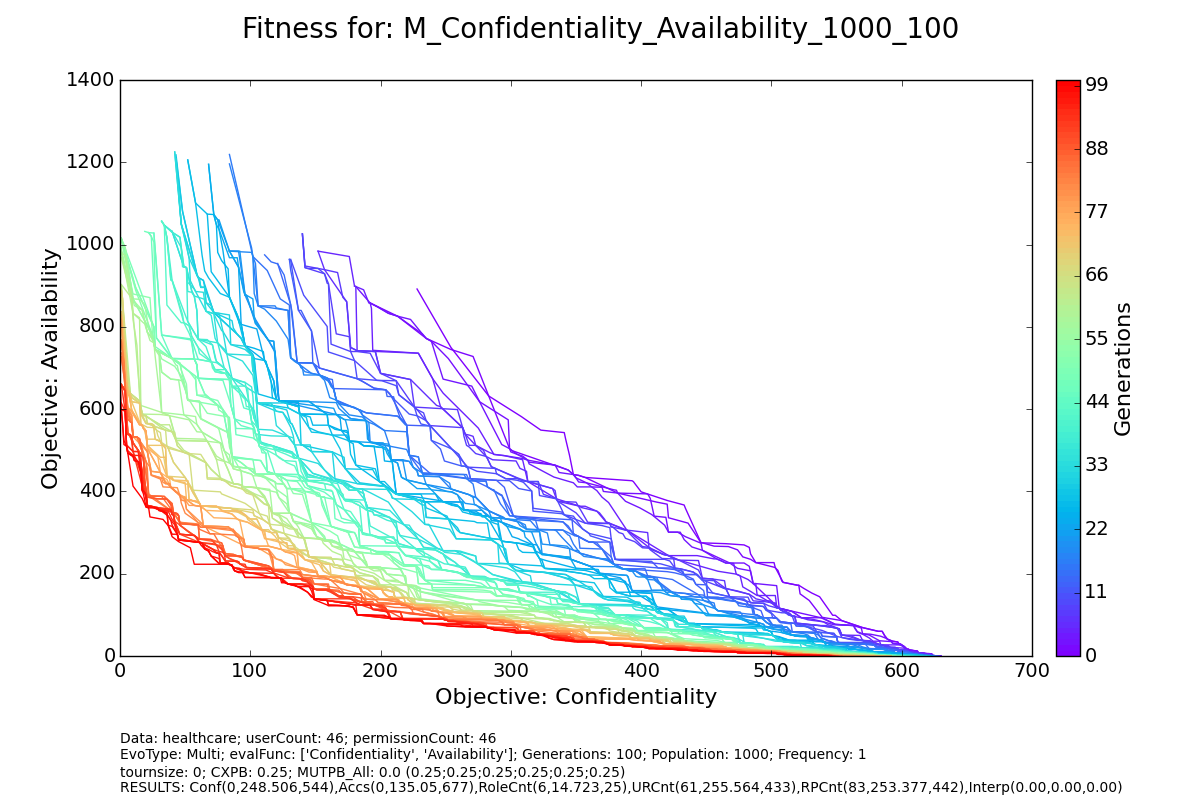
\includegraphics[scale=0.35, trim=0cm 2cm 0cm 1.5cm, clip=true]{exp7_fitness}
	\caption{EXPERIMENT 7: Pareto fronts of each generation in the experiment with EvoRoleMiner$M$ on the healthcare dataset}
	\label{fig:exp7_fitness}
\end{figure}

\begin{figure}[H]
	\centering
	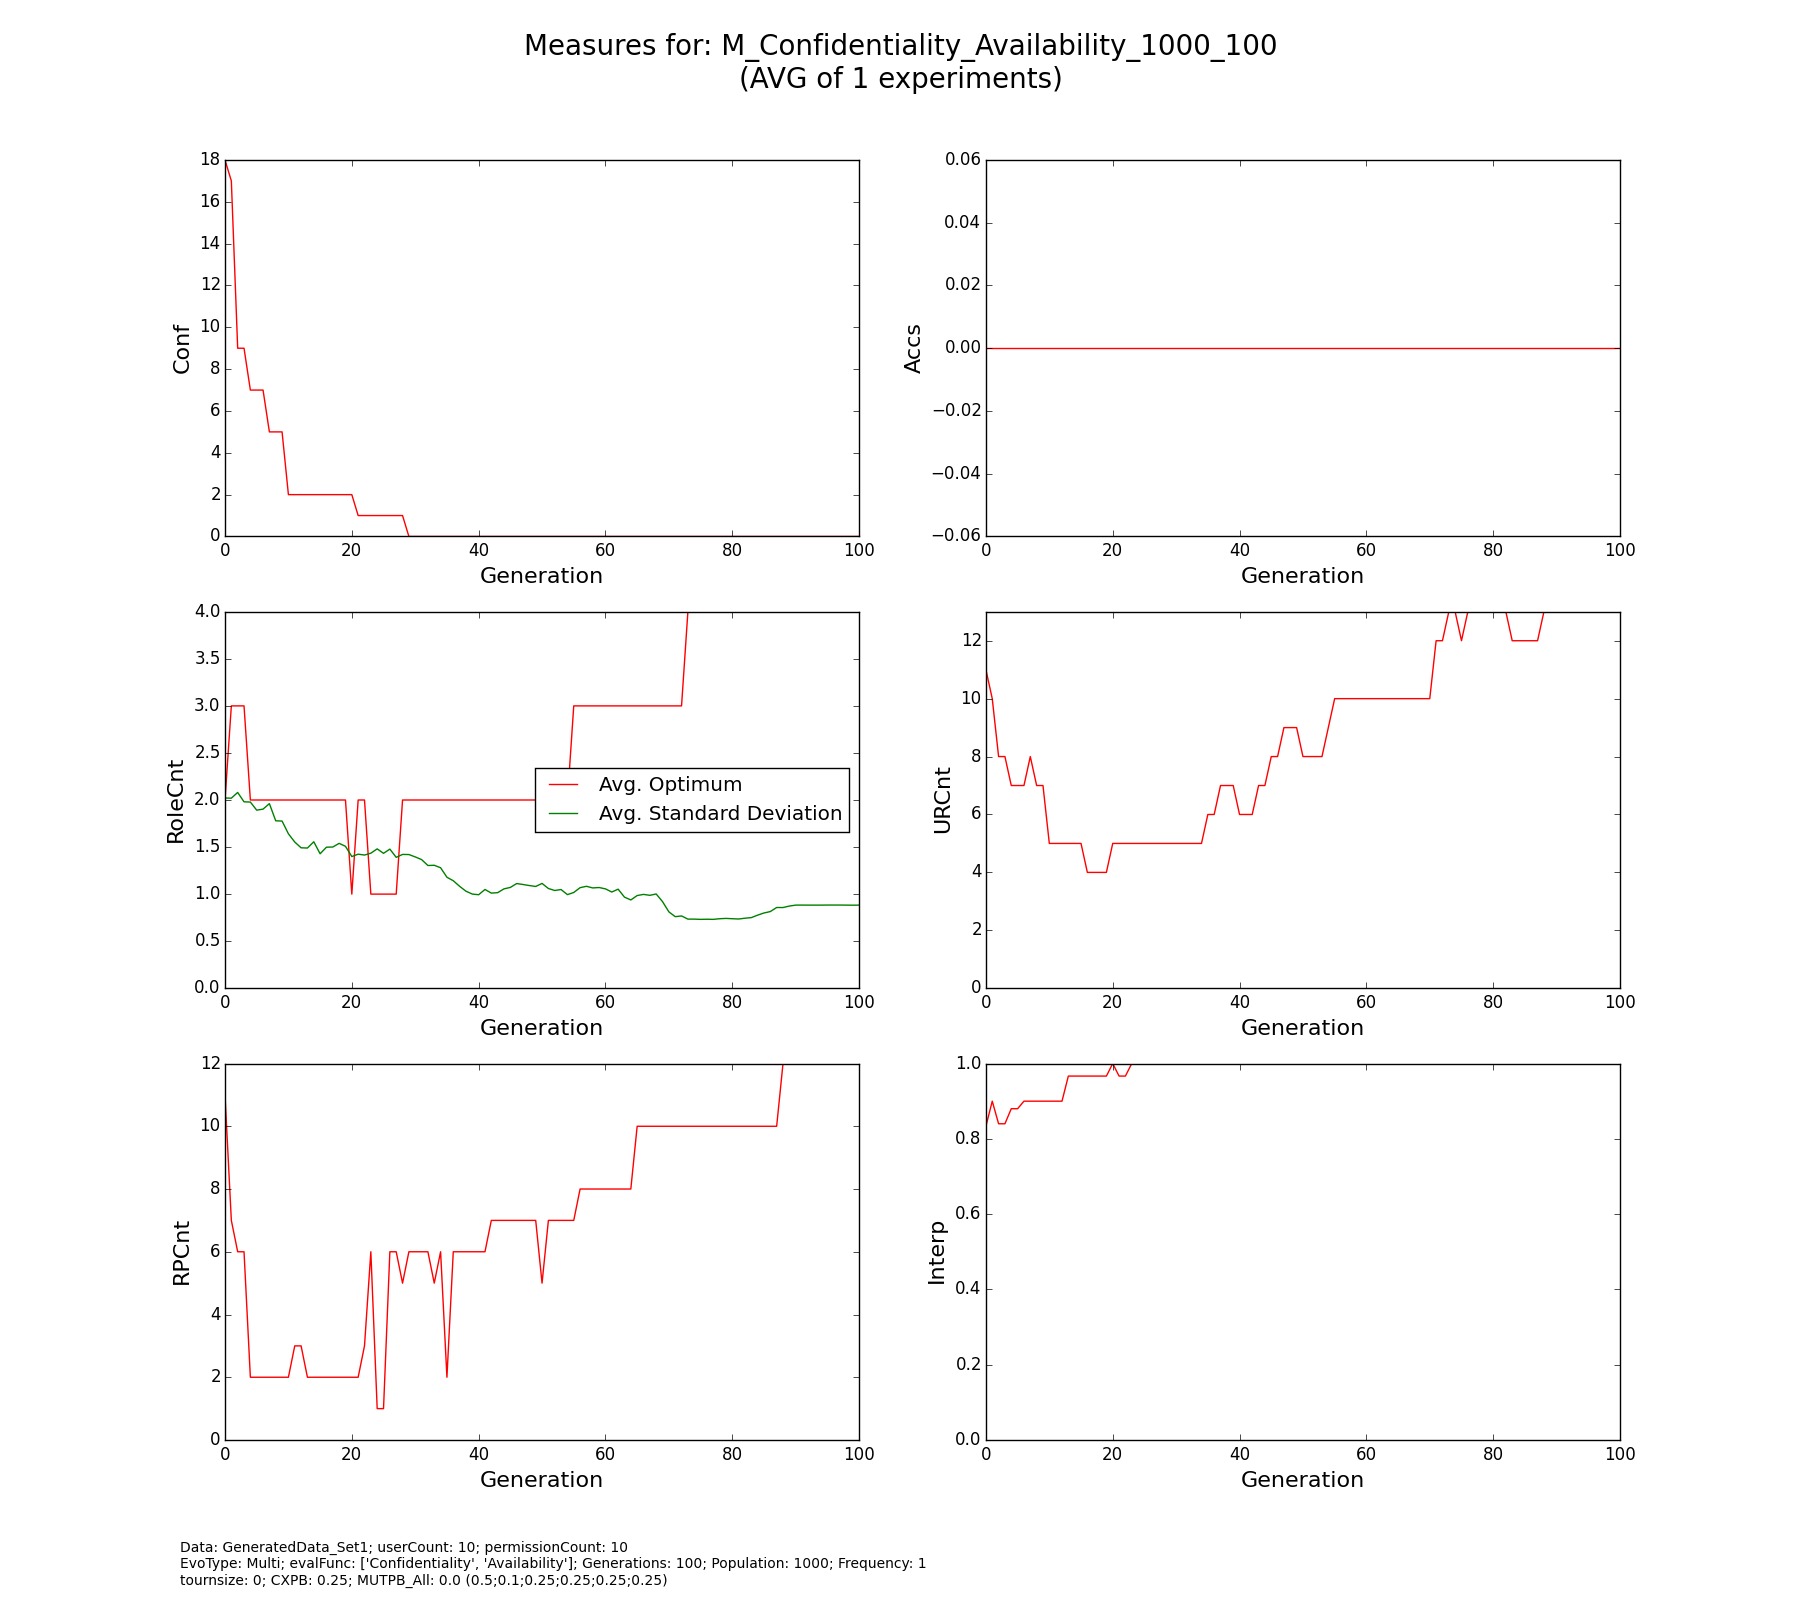
\includegraphics[scale=0.33, trim=4cm 2cm 4cm 0cm, clip=true]{exp6_measures}
	\caption{EXPERIMENT 6: Average optimum of the single objective measures of the ten experiments with EvoRoleMiner$M$ on the synthetic dataset 1}
	\label{fig:exp6_measures}
\end{figure}

\begin{figure}[H]
	\centering
	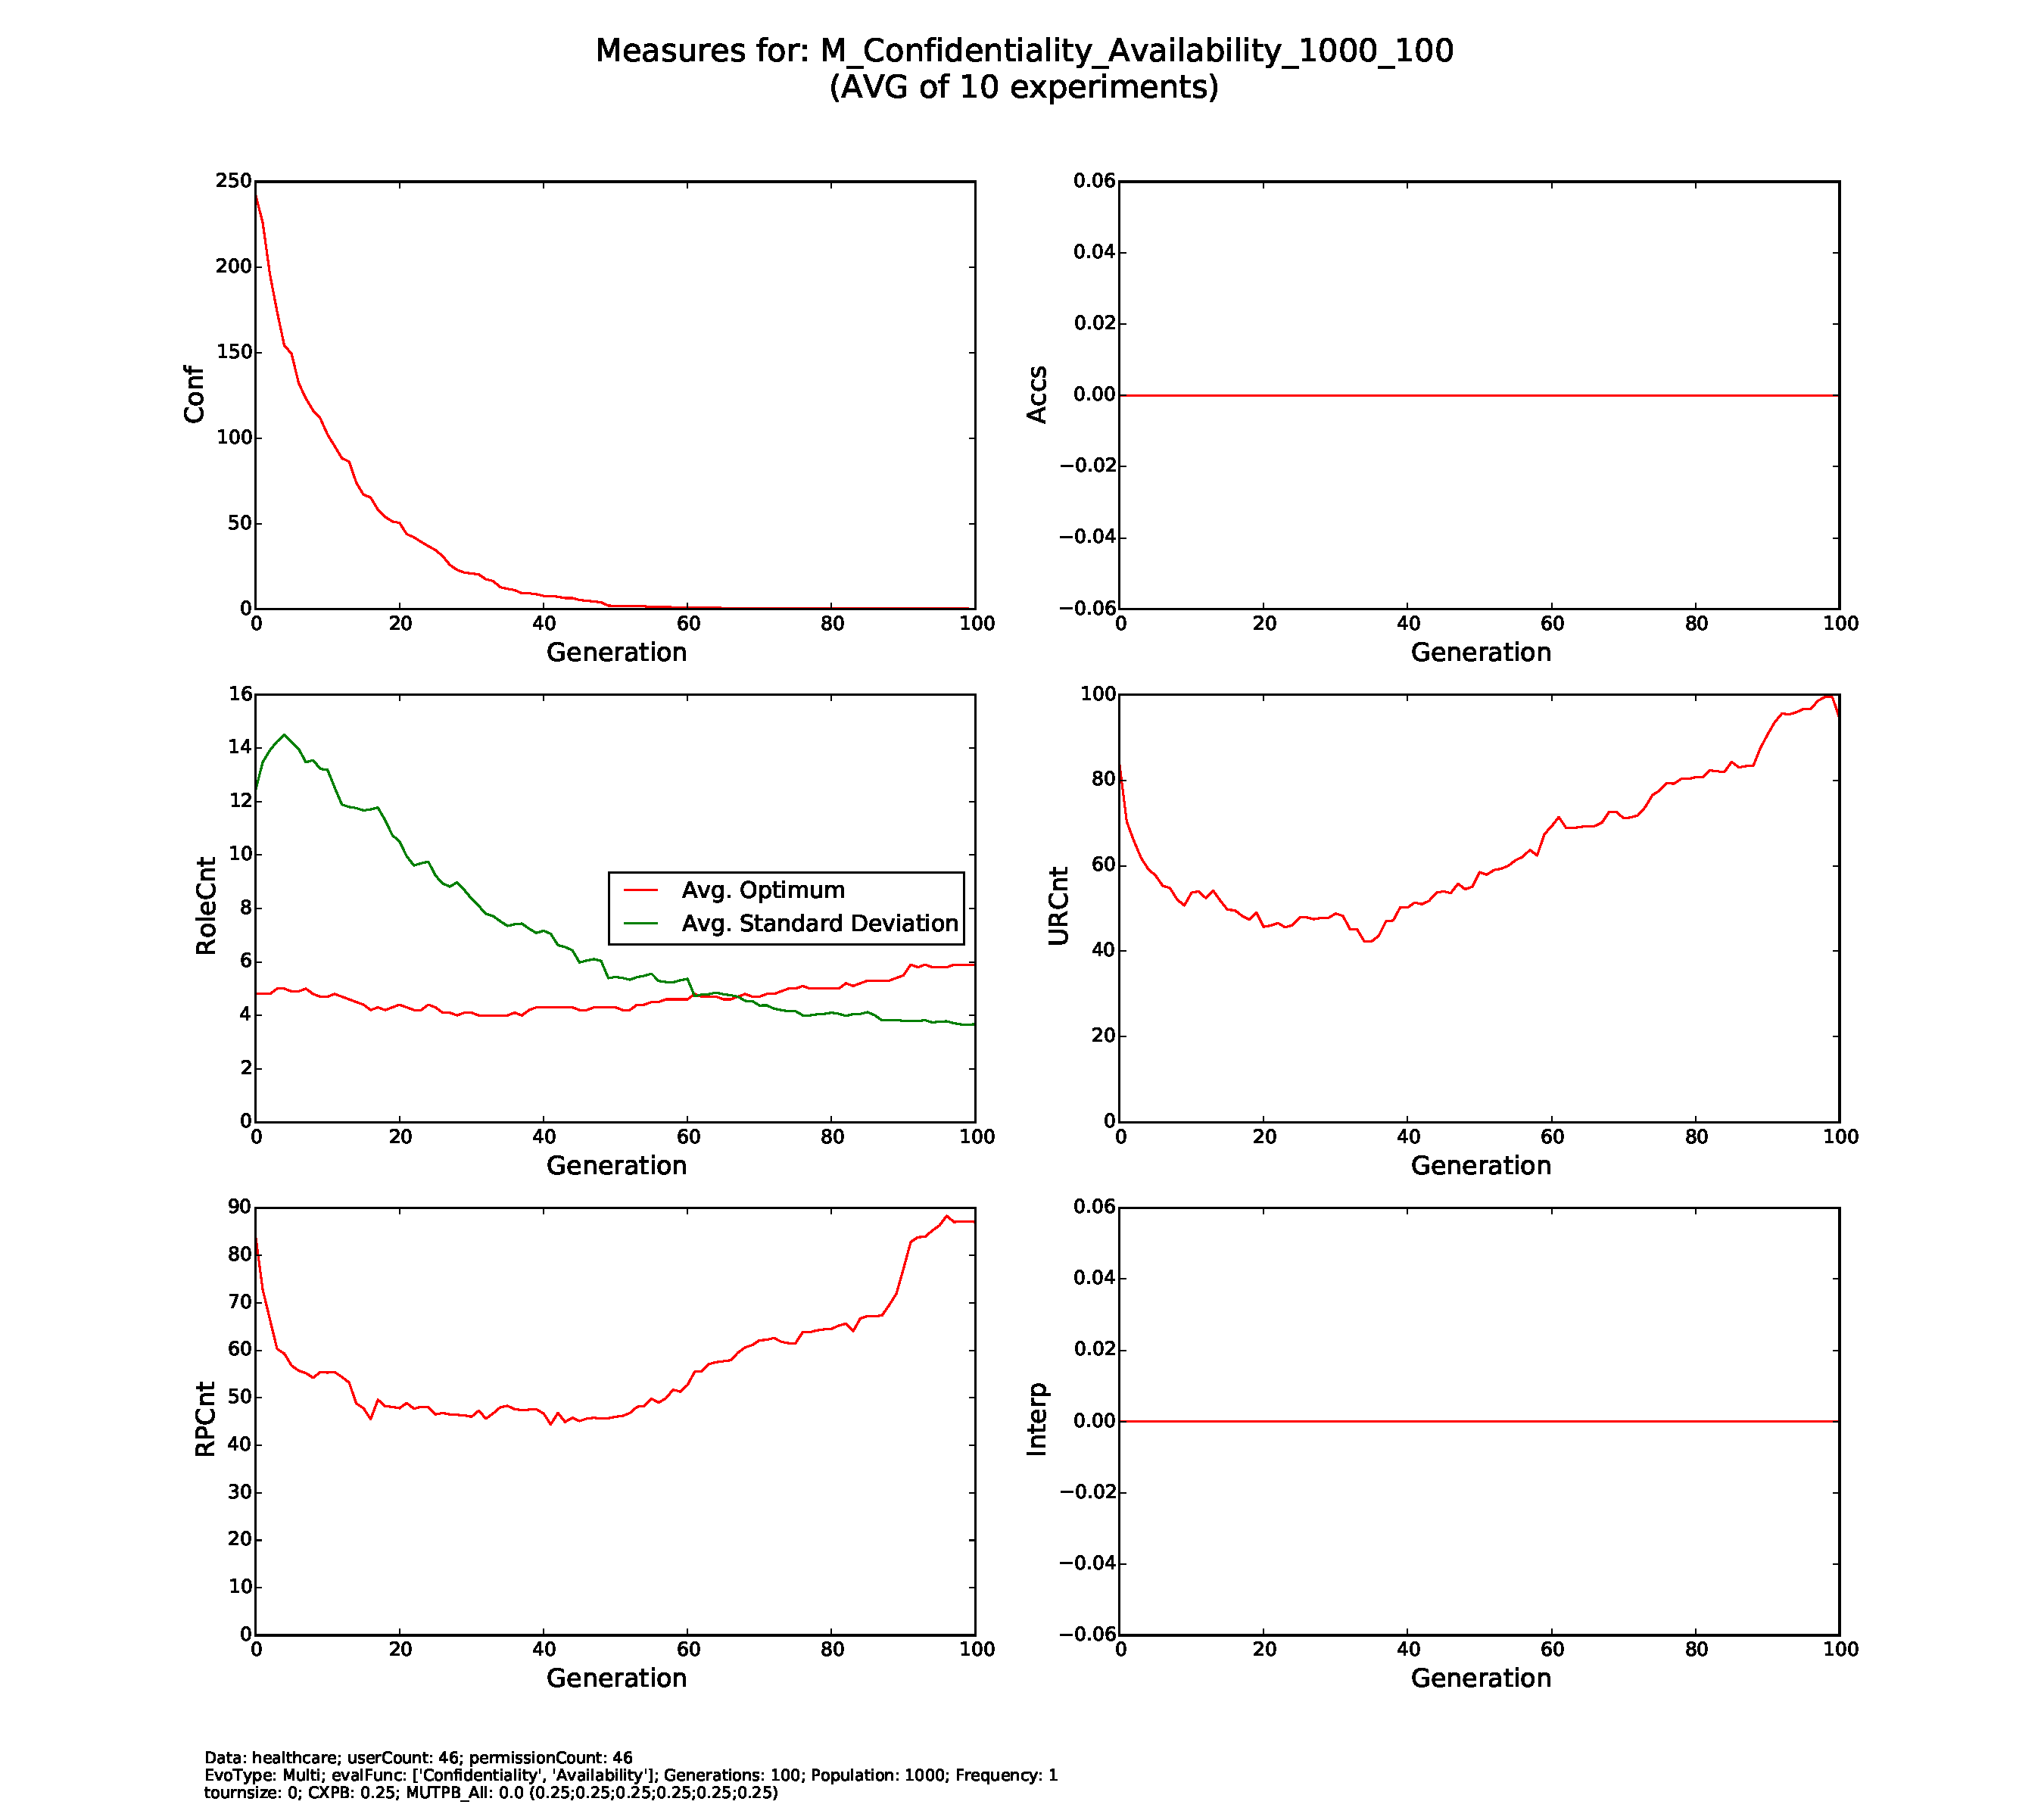
\includegraphics[scale=0.33, trim=4cm 2cm 4cm 0cm, clip=true]{exp7_measures}
	\caption{EXPERIMENT 7: Average optimum of the single objective measures of the ten experiments with EvoRoleMiner$M$ on the healthcare dataset. The Interpretability measure is not activated and therefore constantly zero.}
	\label{fig:exp7_measures}
\end{figure}

Example boxplots on the diversity of the role count of individuals of a population is shown in Figure \ref{fig:exp6_boxplot} for the dataset 1 and Figure \ref{fig:exp7_boxplot} for the healthcare dataset.

\begin{figure}[H]
	\centering
	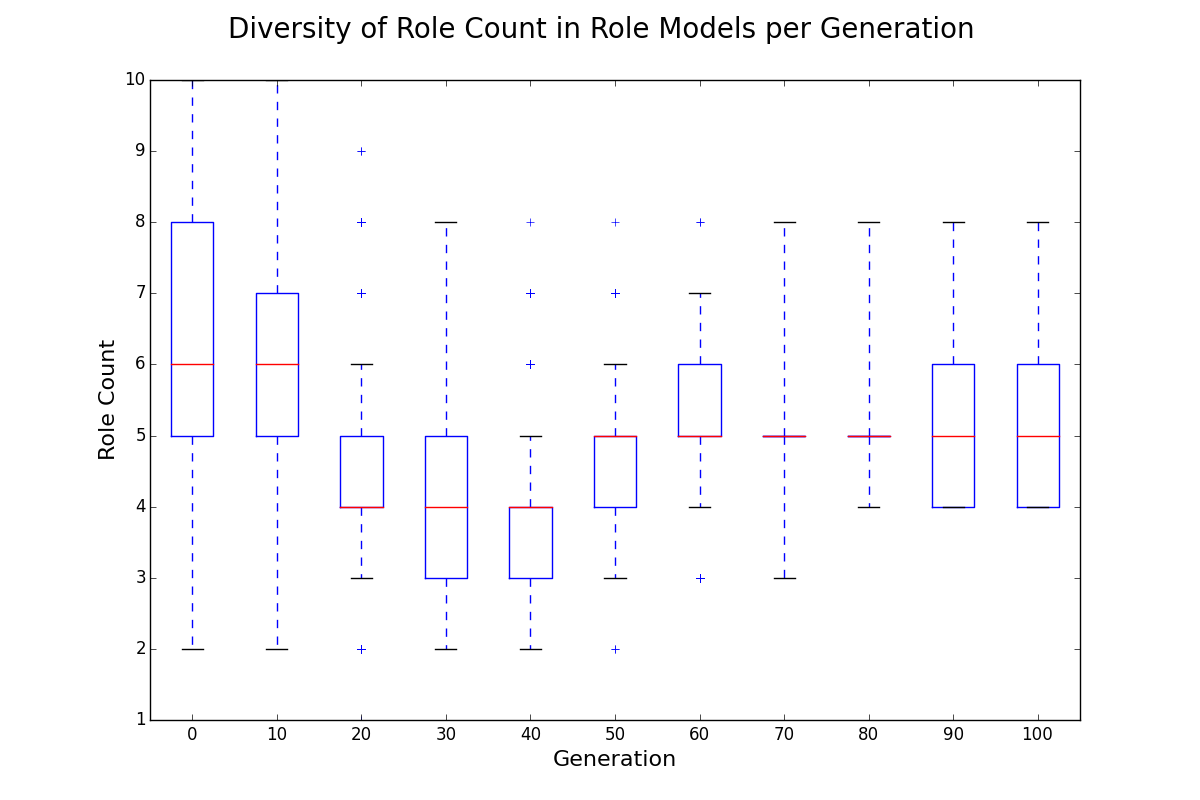
\includegraphics[scale=0.3]{exp6_boxplot}
	\caption{EXPERIMENT 6: Example boxplot of role count diversity of individuals of a population in different generations with EvoRoleMiner$M$ on the synthetic dataset 1.}
	\label{fig:exp6_boxplot}
\end{figure}

\begin{figure}[H]
	\centering
	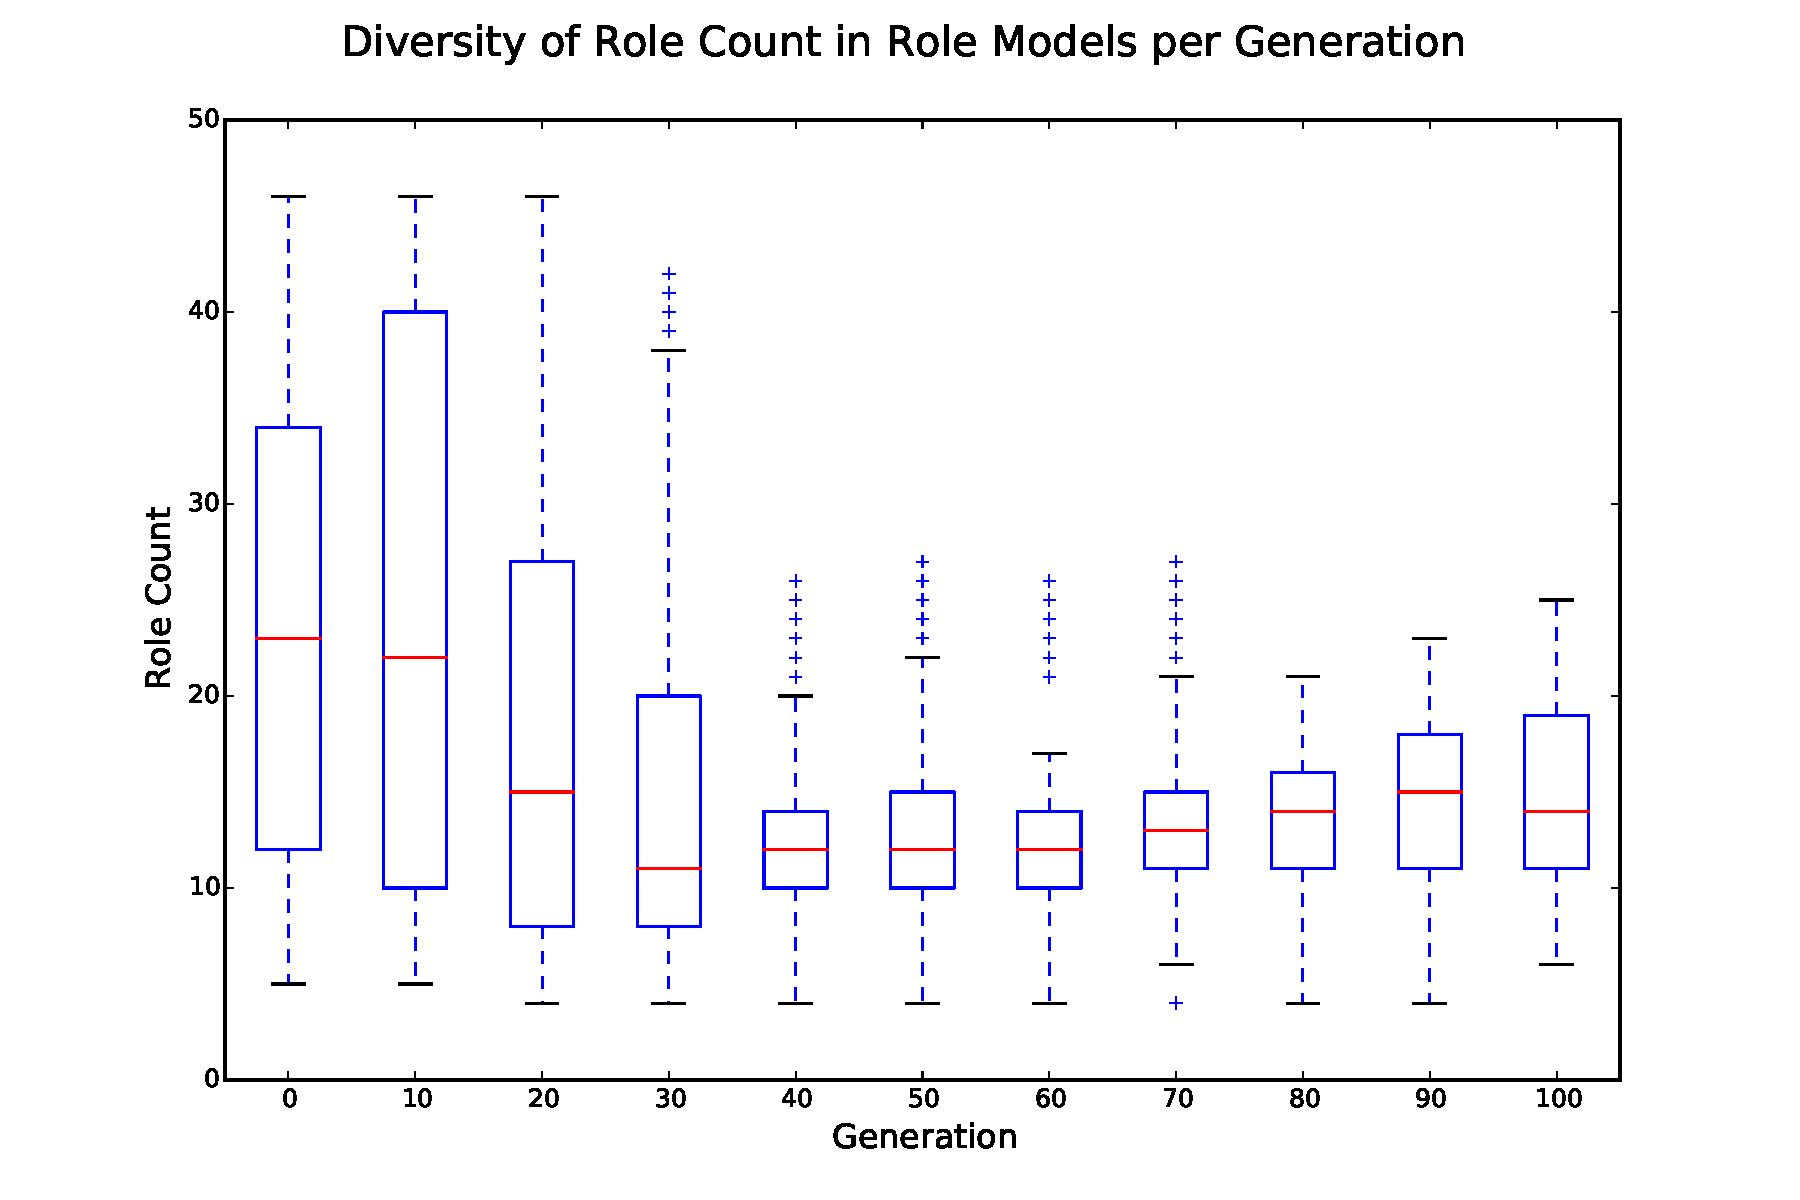
\includegraphics[scale=0.3]{exp7_boxplot}
	\caption{EXPERIMENT 7: Example boxplot of role count diversity of individuals of a population in different generations with EvoRoleMiner$M$ on the healthcare dataset.}
	\label{fig:exp7_boxplot}
\end{figure}